\section{Introdução}\label{introduuxe7uxe3o}

Para a Prática 1 será necessário montar e soldar um circuito numa placa
SanUSB com os seguintes componentes:

\begin{itemize}
\itemsep1pt\parskip0pt\parsep0pt
\item
  1 Micro controlador PIC18F2550
\item
  1 LED
\item
  1 Cristal
\item
  1 Botão de \emph{reset}
\item
  1 resistor $2.2K \Omega$
\item
  1 resistor $390 \Omega$
\item
  2 Capacitores $22pF$
\item
  2 Capacitores $1 \mu F$
\item
  1 Conector USB
\item
  1 Cabo USB
\item
  1 Diodo
\item
  Bournes
\end{itemize}

\section{Objetivos}\label{objetivos}

Fazer com que ao ser alimentado por cabo USB o microcontrolador acione
um LED de modo que ele permaneça piscando.

\begin{figure}[h]
    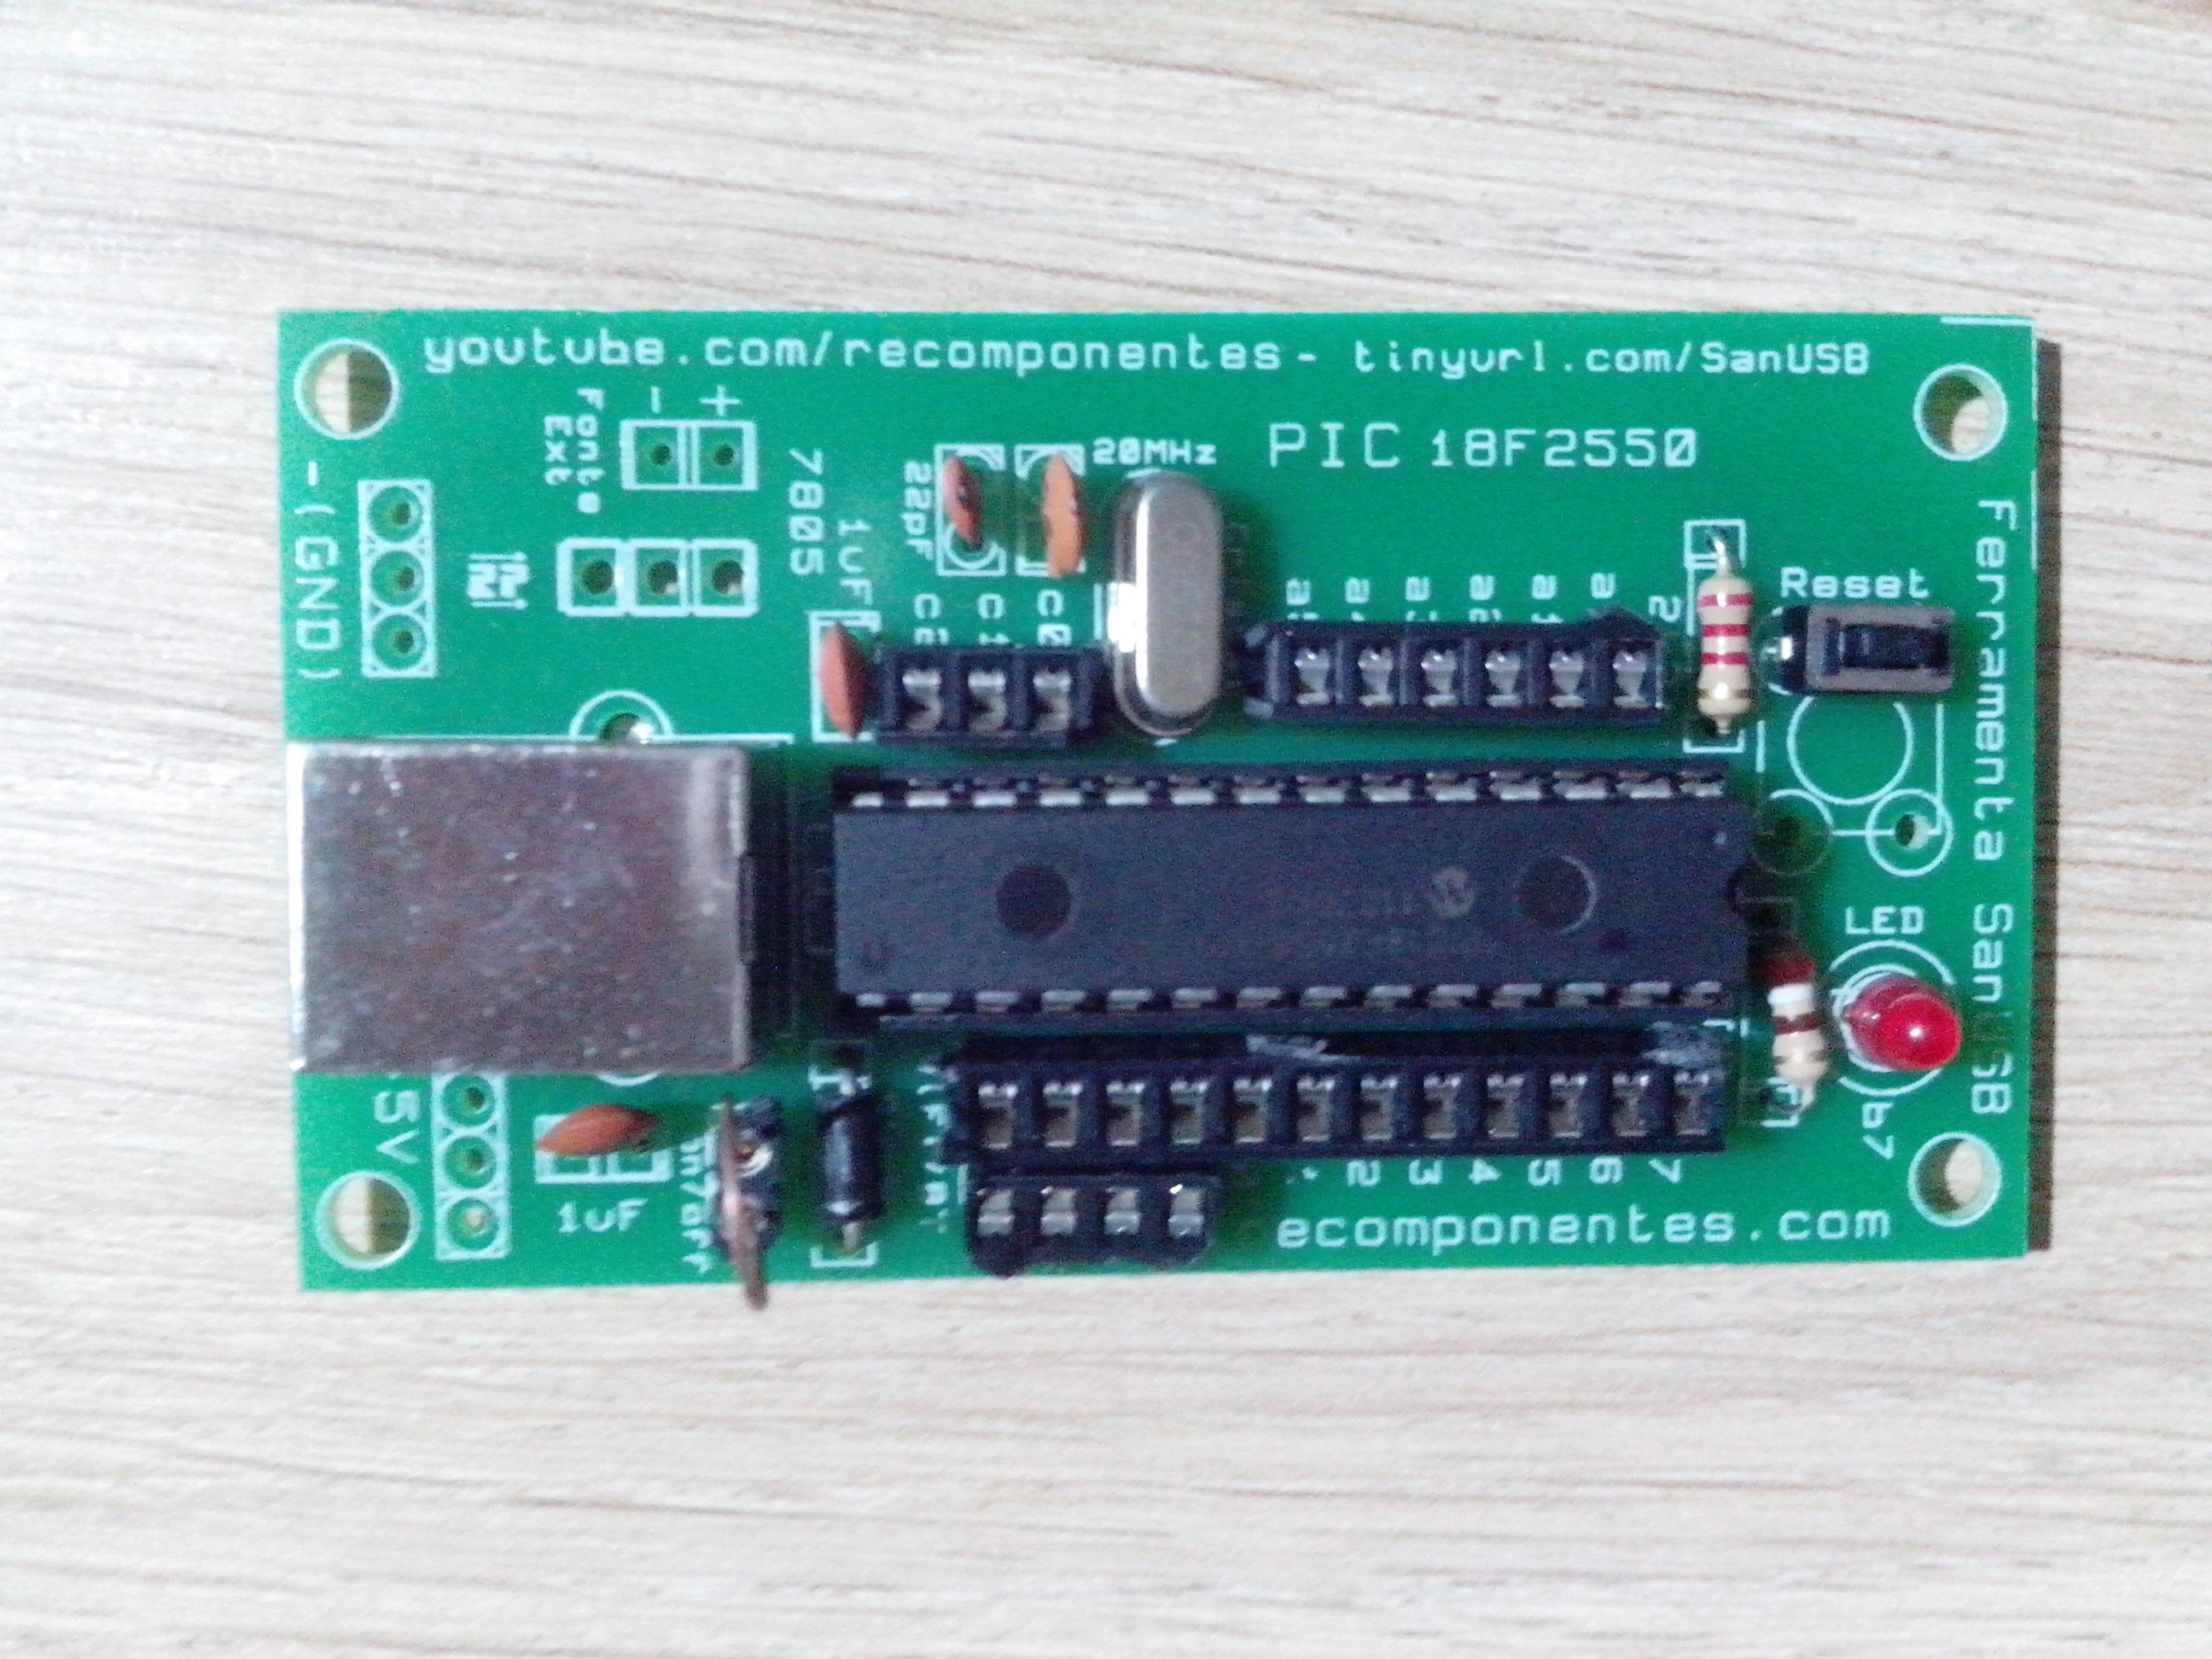
\includegraphics[scale=0.15]{img/placa-1.jpg}
    \caption{Placa montada}
\end{figure}

\section{Conclusão}\label{conclusuxe3o}

A montagem é bem didática por que a placa vem a indicação exata de cada
componente. Além disso a gravação do programa fonte também é facilitada
graças a um programa que envia os dados pela porta USB e reseta o
circuito.

A utilização de porta USB auxilia tanto na gravação quanto na
alimentação do circuito, visto que é um componente barato e que toda
máquina moderna possui por padrão.
